%! alt Square ABCD with side 12, A at the bottom left, B at the bottom right, C at the top right and D at the top left. E is on BC with BE = 4 and F is on CD with DF = 6, so angle EAF is 45 degrees. Rotating F by 90 degrees about A gives G on line CB beyond B, with BG = 6. Triangle AEF is highlighted and is congruent to the dashed triangle AGE, and EF = GE = 10.
%! after_paragraph 1
%! scale 2/7
% The shared preamble of every Cevian figure. pipeline/figures turns these colours into theme-aware paint,
% and refuses any other colour, so draw only with them:
%   figink (lines and labels), figaux (construction lines), figaccent (the object the argument turns on),
%   figtint and figaccenttint (light fills).
\documentclass[border=1.5pt]{standalone}
\usepackage{tkz-euclide}
\definecolor{figink}{RGB}{0,0,0}
\definecolor{figaux}{RGB}{85,85,85}
\definecolor{figaccent}{RGB}{192,57,43}
\definecolor{figtint}{RGB}{221,221,221}
\definecolor{figaccenttint}{RGB}{245,213,208}
% tkz-euclide's defaults draw circles, compasses and marks in 50% grey and fill points with a tint.
\makeatletter
\def\tkz@otherlinecolor{figink}
\def\tkz@euc@circlecolor{figink}
\def\tkz@euc@compasscolor{figink}
\def\tkz@euc@mkcolor{figink}
\def\tkz@mk@fill{figink}
\def\tkz@euc@pointfillcolor{figink}
\makeatother
\tkzSetUpLine[color=figink,line width=.7pt]
\tkzSetUpArc[color=figink,line width=.7pt]
\tkzSetUpCompass[color=figink,line width=.5pt]
\tkzSetUpPoint[color=figink,fill=figink,size=3.1pt]
\tikzset{
  every picture/.style={line cap=round,line join=round,color=figink},
  circle style/.append style={color=figink,line width=.7pt},
  aux/.style={color=figaux,line width=.45pt,dash pattern=on 2.6pt off 2pt},
  key/.style={color=figaccent,line width=1pt},
  mk/.style={color=figink,line width=.5pt},
  lbl/.style={color=figink,inner sep=2.2pt},
  len/.style={color=figink,inner sep=1.5pt,font=\small},
}

\begin{document}
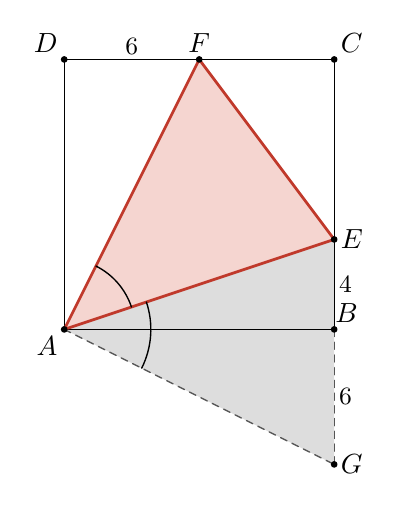
\begin{tikzpicture}
\tkzDefPoint(0.0,0.0){A} %! A = (0, 0)
\tkzDefPoint(3.4285714,0.0){B} %! B = (12, 0)
\tkzDefPoint(3.4285714,3.4285714){C} %! C = (12, 12)
\tkzDefPoint(0.0,3.4285714){D} %! D = (0, 12)
\tkzDefPoint(3.4285714,1.1428571){E} %! E = (12, 4)
\tkzDefPoint(1.7142857,3.4285714){F} %! F = (6, 12)
\tkzDefPoint(3.4285714,-1.7142857){G} %! G = rotate(F, A, -90)
%! fact angle(E, A, F) == 45
%! fact angle(G, A, E) == 45
%! fact equal(dist(A, G), dist(A, F))
%! fact collinear(G, B, C)
%! fact dist(B, G) == 6
%! fact dist(E, F) == 10
%! fact dist(G, E) == 10
%! fact area(A, E, F) == 60
\tkzFillPolygon[color=figaccenttint](A,E,F)
\tkzFillPolygon[color=figtint](A,G,E)
\tkzDrawPolygon(A,B,C,D)
\tkzDrawPolygon[key](A,E,F)
\tkzDrawSegments[aux](A,G B,G)
\tkzMarkAngle[size=.9,arc=l,mark=none,mk](E,A,F)
\tkzMarkAngle[size=1.1,arc=l,mark=none,mk](G,A,E)
\tkzDrawPoints(A,B,C,D,E,F,G)
\tkzLabelPoint[below left,lbl](A){$A$}
\tkzLabelPoint[above right,xshift=-2pt,lbl](B){$B$}
\tkzLabelPoint[above right,lbl](C){$C$}
\tkzLabelPoint[above left,lbl](D){$D$}
\tkzLabelPoint[right,lbl](E){$E$}
\tkzLabelPoint[above,lbl](F){$F$}
\tkzLabelPoint[right,lbl](G){$G$}
\tkzLabelSegment[right,len](B,E){$4$}
\tkzLabelSegment[above,len](D,F){$6$}
\tkzLabelSegment[right,len](B,G){$6$}
\end{tikzpicture}
\end{document}
